\documentclass[11pt]{article}
\usepackage{amssymb}
\usepackage{amsmath}
\usepackage{graphicx}
\usepackage{fullpage}
\usepackage{gensymb}
\usepackage{float}
\usepackage{upgreek}
\usepackage{hyperref}
\graphicspath{ {C:\Users\Dat\Documents\GitHub\Arduino\exp10-diy-arduino} }
\usepackage[margin=2cm]{geometry}
\tolerance=1000
\date{}
\title{Building Your Own Arduino}
\begin{document}
\maketitle
	
\centerline{
	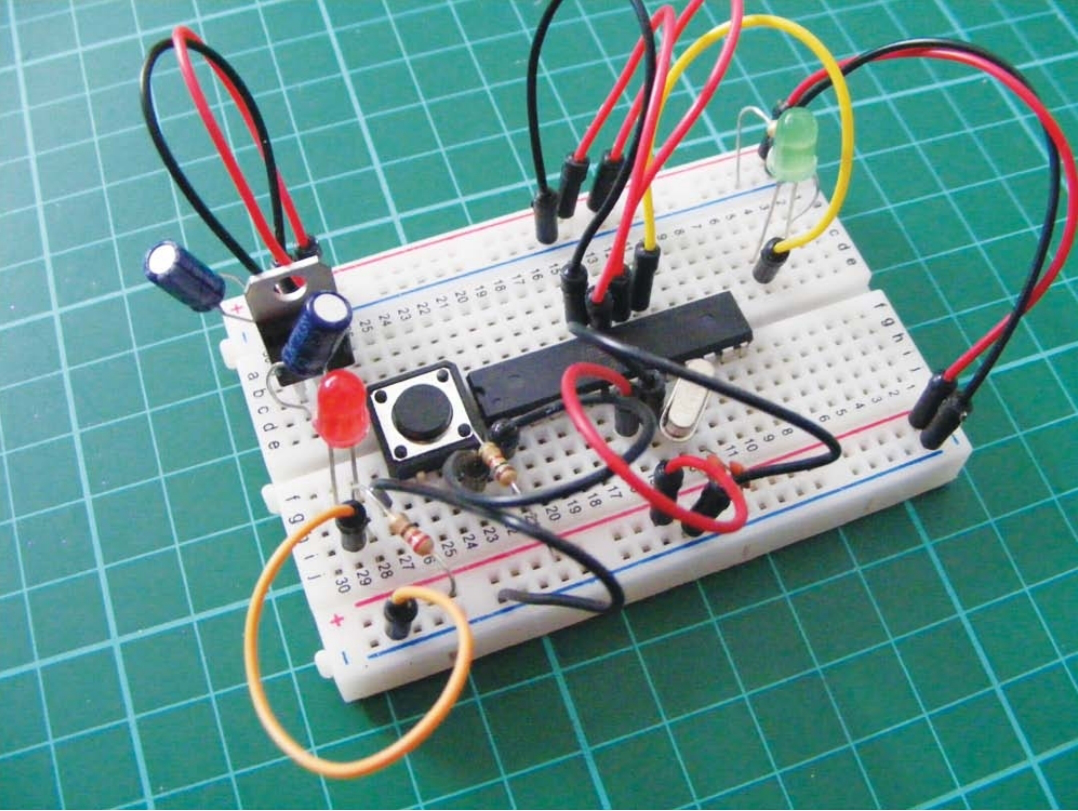
\includegraphics[scale=.55]{exp10-board}	
}

\section{Setup}
\label{sec-1}

First you will need to download, unzip, and install the Arduino Integrated Development Environment (IDE) from
\url{https://www.arduino.cc/en/Main/Donate} (does not need admin privileges).

\section{How it works}
\label{sec-2}
The custom Arduino is meant to be able to replicate the functionality of a Arduino board. The custom board utilizes the ATMEL ATmega328p chip. This is a chip that sits on the pre-built Ardunio board and must be programmed on the board via USB prior to utilization on the custom board. This chip contains the brains of the Arduino. The layout of the chip including the pins and their functions can be seen below. 

\centerline{
	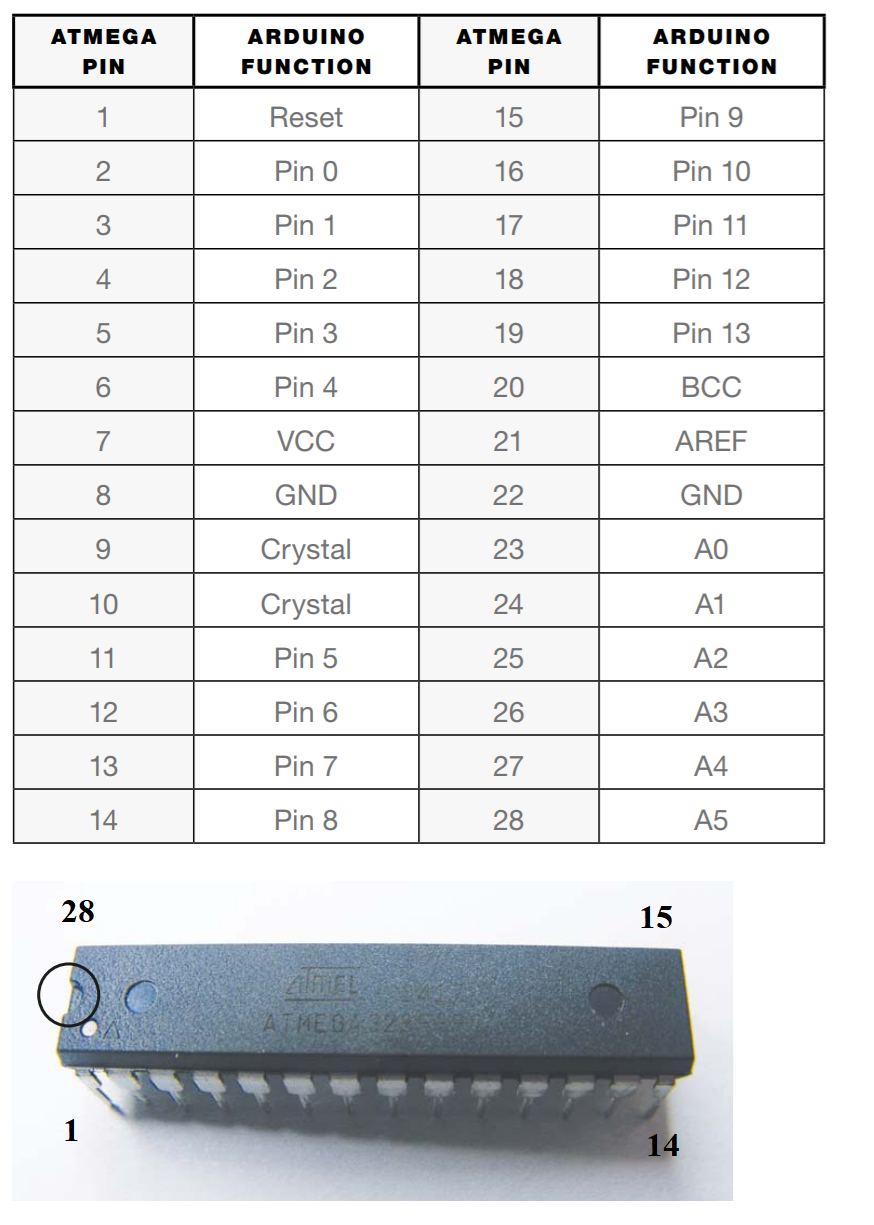
\includegraphics[scale=1]{exp10-pin}	
}

In addition to the ATmega chip, there are several other aspects that are important to the custom board. This includes a 5V regulator to limit the 9V battery to the operating voltage of the ATmega chip, 5V. A crystal oscillator is used to control the timing of the Arduino. The on and off switch is also replaced by pushbutton while two color leds are used for indication of power and status.

\section{Building The Circuit}
\label{sec-3}

The schematics for the circuits you will be building is below.

\centerline{
	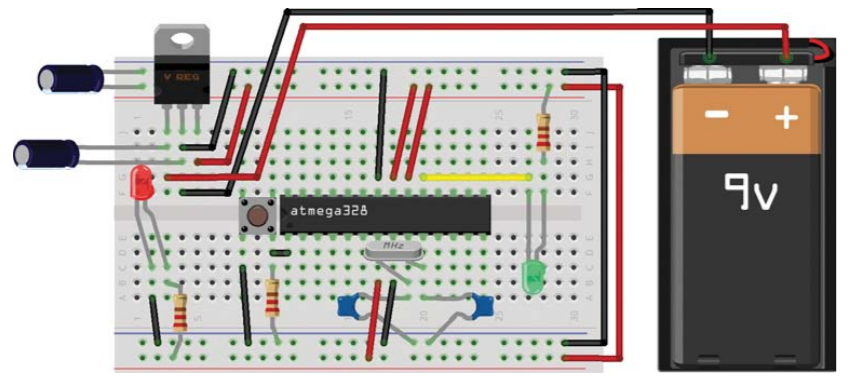
\includegraphics[scale=2]{exp10-schematics}	
}

\section{Programming the Arduino}
\label{sec-4}
In order to program the Arduino, the ATmega chip must be transfer back to the custom board. After the ATmega chip is back in the Arduino board, connect the board to the computer via usb and programmed the board. 

A simple blinking LED code for programming the Arduino is provided. Using the Arduino IDE, open the .ino file.
The IDE allows you to do 4 things: edit the code, verify the code is correct (i.e. does not contain
syntax errors), upload the code to the Arduino, and view the diagnostic output of things as they run on
the Arduino.
Uploading to the Arduino is easy! Just click the Upload arrow in the IDE. 

After the board is successfully programmed, the Arduino board can be disconnected from the computer and transfered back to the custom board. The program should now be uploaded and function as expected on the custom board.

\section{The Code}
\label{sec-5}
A simple blinking LED code is provided to verify the functionality of the custom built Arduino. This code uses pin 13 of the Arduino function and should make the corresponding LED blink on the custom board. 

\section{Going Further}
\label{sec-6}
Now that the board's functionality is verified, the board is able to accomplish anything a Arduino board can after a successful upload. The battery allows the custom board to be used without a connected computer. 

\begin{itemize}
	\item Upload and run Arduino projects that you have used in the past. Just remember to upload the code on the board prior to the custom board and be wary of the pin layout. 
	
	\item Build a custom container for the custom Arduino for easier carrying. You could even try to replace the bread board with soldering. 
\end{itemize}

\end{document}

